

\chapter*{\centering\large{3. Исследование факторов, влияющих на точность программно-имитационной модели системы связи}}
\addcontentsline{toc}{chapter}{3. Исследование факторов, влияющих на точность программно-имитационной модели системы связи}	
\label{sec:Chapter3} \index{Chapter3}

\section*{\large{3.1 Метод анализа результатов моделирования}}
\addcontentsline{toc}{section}{3.1 Метод анализа результатов моделирования}

\begin{onehalfspace}
    В моделируемом примере приёмники и передатчики каналов <<базовая станция — ретранслятор>> и <<абонент — ретранслятор>> глобально не разнесены в пространстве и взаимно влияют на организацию каналов передачи друг друга. Так, если в каналах <<базовая станция — ретранслятор>> изменяется мощность передачи сигнала, то  и  в соответствующих каналах  <<абонент — ретранслятор>> и  <<абонент — ретранслятор>>  и <<базовая станция — ретранслятор>> тоже меняется качество сигнала и время его передачи внутри канала связи. В таком случае возникает задача моделирования процесса передачи данных, с учётом влияния на сигнал накладывания собственных копий сигнала с разными фазами, это связано с многолучевым распространением сигнала из-за того, что путь распространения радиоволны между передатчиком и приёмником радиоволны не определён однозначно, из-за неоднородности среды распространения и наличия огибаемых и отражающих препятствий.



    Рассматриваемый процесс передачи данных в канале <<базовая станция - ретранслятор — абонент>> моделируется передачей ping-сигнала от базовой станции к абоненту. Критерием качества является совпадение данных из полученного от абонента, повторённого на ретрансляторе, сигнала и данных, в сообщении отправленном базовой станцией. Проверка происходит в блоке обработки данных (блок $Data \ Verification$ аналогично 2.2 Структура модели базовой станции). Для учёта влияния задержек, появляющихся в следствие устройства модели, которые описаны на рисунке 4, используется линия валидности сигнала (2.5 Описание принципа учёта задержек системы ретрансляции п.3), которая на каждом блоке (к примеру, фильтре) соответствующего модуля (к примеру, базовая станция) сравнивает ожидаемое значение и текущее, что позволяет определить задержку, получаемую в данном блоке. 
    

    Определяющими параметрами модели являются частоты, амплитуды, режим модуляции и скорости передачи данных. Помимо этого, модель построена так, что позволяет изменять канал передачи, к примеру, добавлением модели шума. Тогда появляется возможность изучить работу модуля одиночно или в комплексе при наличии сильно зашумленных сигналов, которые, к тому же, достигли входа уже после многократного переотражения. Модель позволяет добавлять имитационные модули отдельных процессов и проверять их влияние на исследуемые параметры системы. Так можно моделировать передачу данных и потери полезной информации вовремя передачи по канала в диапазонах высоких частот. На рисунке 16 изображена разработанная в Simulink модель системы «базовая станция – ретранслятор – абонент», учитывающая фазовые и частотные искажения сигналов, а также ослабления сигналов в канале связи.

 \begin{figure}[h!]
\centering
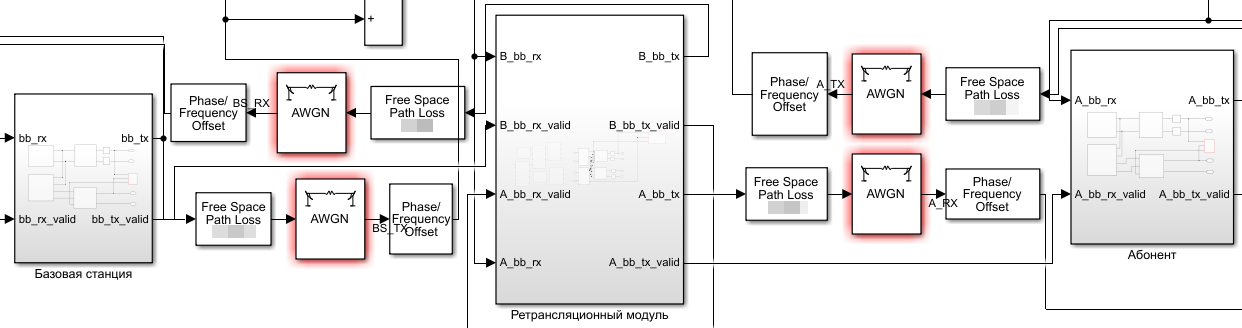
\includegraphics[width=1\linewidth]{bigger6.png}
\caption{Модель системы «базовая станция – ретранслятор – абонент» в Simulink}
\label{fig:model22}
\end{figure}


\end{onehalfspace}

	\section*{\large{3.2 Результаты моделирования базовой станции}}
 \addcontentsline{toc}{section}{3.2 Результаты моделирования базовой станции}
\begin{onehalfspace}
    Исследуемым параметром является принятый сигнал на модуле базовой станции, который может за счёт переотражений порождать паразитные сигналы, с различными значениями амплитуды и фазы, являющиеся копиями самого сигнала, которые влияют на качество итогового принятого сигнала. Отследить это влияние можно сравнением одиночной работы модуля в режиме одновременного приёма и передачи, а также работы в комплексе с остальными модулями. Рисунок 17 демонстрирует эти результаты для первого описанного случая, также он отображает соответствие модельных данных значения BER ожидаемым теоритическим, в канале $bb\_tx - B\_bb\_rx$ ($bb\_tx\_valid - bb\_rx\_valid$), с помощью расчёта показателя достоверности приема двоичных символов, используемый для оценки качества каналов связи, с помощью инструмента bertool(Matlab+Simulink), настроенного под параметры модели.
\end{onehalfspace}
	
	\begin{figure}[h]
		\begin{minipage}[h]{0.49\linewidth}
			\center{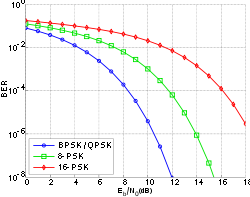
\includegraphics[width=0.7\linewidth]{BER_wiki.png} \\ Теоретическая зависимость}
		\end{minipage}
		\hfill
		\begin{minipage}[h]{0.49\linewidth}
			\center{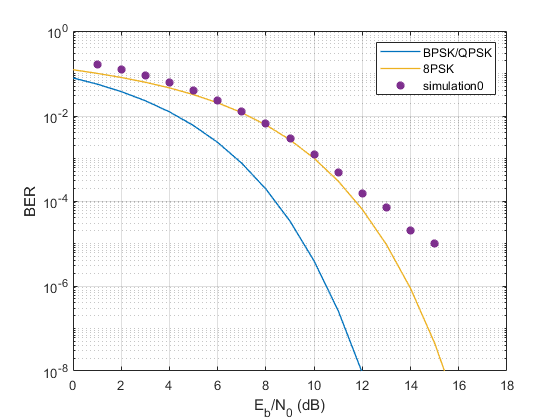
\includegraphics[width=0.8\linewidth]{realPSK.png} \\ Модель базовой станции}
		\end{minipage}
		\caption{Вероятность ошибки на бит (BER) в зависимости от $\frac{Eb}{N0}$ в dB}
		\label{fig:model20}
	\end{figure}

\begin{onehalfspace}
Параметр BER представляет собой метрику, которая определяет вероятность ошибочного приема битовой последовательности в канале связи. То есть, BER показывает частоту возникновения ошибки в передаче данных по радиоканалу, также он является показателем качества связи в канале <<базовая станция — ретранслятор>>, чем ниже значение BER, тем лучше качество связи. 


Также качественное соответствие принятого и полученных сигналов можно отследить через спектры сигналов и состояние QPSK-созвездий, на которых также можно видеть влияние шума (моделируемого АБГШ) и внешних факторов, влияющих на канал <<базовая станция — ретранслятор>> . Рисунок 18 демонстрирует спектры сигналов при моделировании сценария ping, с компенсацией задержек за счёт внутреннего устройства модуля (фильтры, модулирующие блоки), полученной в канале валидности $B\_bb\_tx\_valid - bb\_rx\_valid$.
\end{onehalfspace}

\begin{figure}[h]
		\begin{minipage}[h]{0.49\linewidth}
			\center{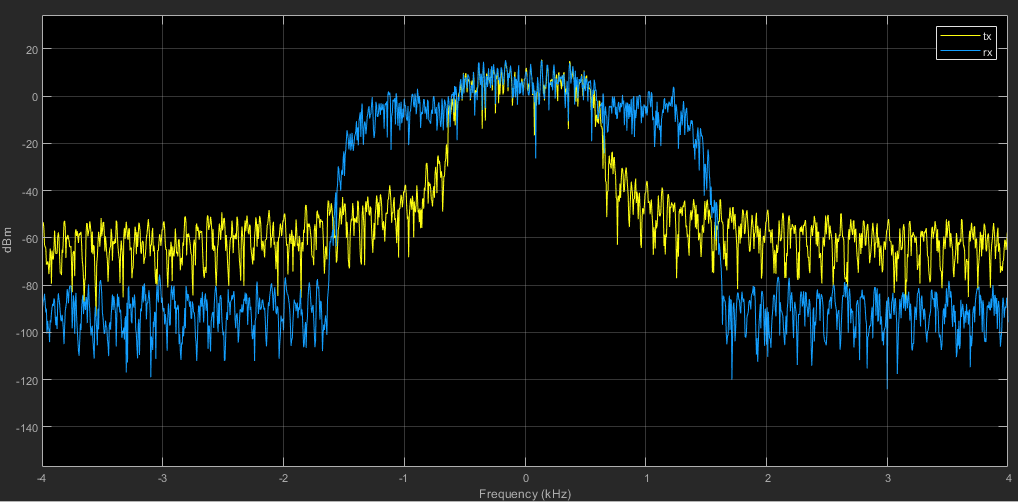
\includegraphics[width=0.7\linewidth]{base_spec.png} \\  Спектры принятого и отправленного ping-сигнала базовой станции}
		\end{minipage}
		\hfill
		\begin{minipage}[h]{0.49\linewidth}
			\center{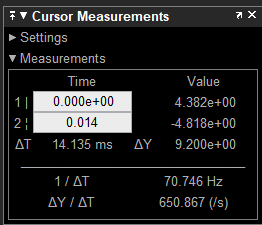
\includegraphics[width=0.6\linewidth]{base_det.png} \\ Временные задержки модели, полученные мониторингом линии валидности}
		\end{minipage}
		\caption{Результат моделирования сигнала на модуле базовой станции}
		\label{fig:model21}
	\end{figure}


\begin{onehalfspace}
В целом, параметр BER является ключевым индикатором при моделировании радиосвязи и позволяет оценить эффективность и надежность передачи данных в радиоканале. Моделирование позволяет исследовать влияние различных факторов на BER, таких как шум, потери сигнала, интерференция и другие искажающие эффекты. 


Однако вышеперечисленные эффекты влияют на спектр принятого сигнала, что даёт неточность обработки принятой информации, для минимизации ошибок, необходимо также следить за спектром сигнала. Анализ спектра может помочь идентифицировать и оценить эти искажения и принять меры по их устранению или снижению. Также с помощью спектра можно определить характеристики сигнала, такие как гармоники, синхропосылки, межсимвольные интерференции и другие параметры, которые могут быть важными при анализе и обработке сигнала.

\end{onehalfspace}



\section*{\large{3.3 Результаты моделирования процесса ретрансляции}}
\addcontentsline{toc}{section}{3.3 Результаты моделирования процесса ретрансляции}
\begin{onehalfspace}

Одним из основных приложений данной модели является имитация процесса повторения сигнала, направленного от базовой станции к абоненту через ретранслятор и, аналогично, от абонента к базовой станции. Ретранслятор имеет в своей зоне видимости оба модуля абонента и ретранслятора, которые не находятся в зоне видимости друг друга. Ретранслятор выполняет функцию усиления слабого полезного сигнала, полученного от базовой станции, перед его передачей абоненту. Таким образом, модель может быть применима для оценки качества передачи сигнала, между модулями канала <<базовая станция — ретранслятор — абонент>>, при заданных положениях в пространстве. 


Также важным является согласование каналов связи (приёма и передачи) текущих потребителей. В данном примере моделирования ping-сигнала, при условии недостаточного усиления сигнала в канале <<абонент — ретранслятор>> рисунок 19 демонстрирует вид спектров сигналов (TX — абонент, RX — базовая станция), обрабатываемых на ретрансляторе. Исследование BER помогает оптимизировать производительность системы и достичь требуемого уровня качества связи, это важно при моделировании как ping-сигналов, помогающих определить минимально время связи между модулями системы, так и пакетной передачи данных. 

\end{onehalfspace}

 \begin{figure}[h!]
\centering
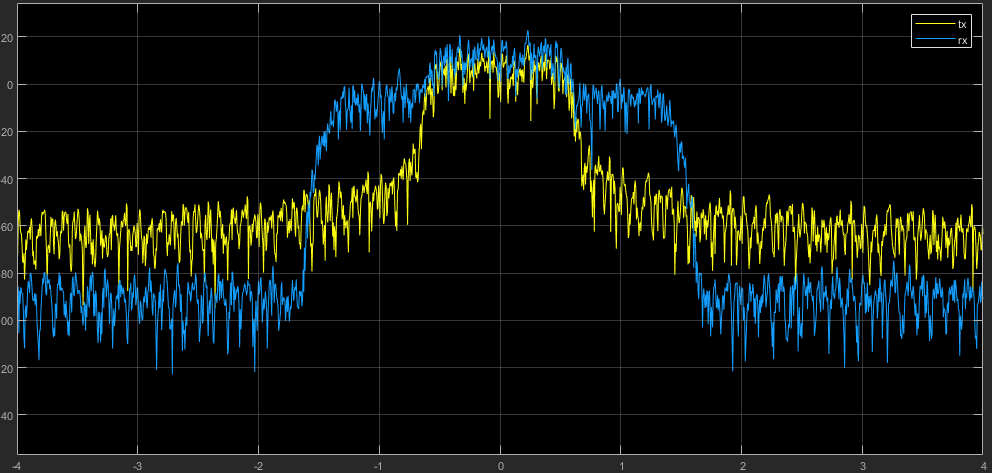
\includegraphics[width=0.9\linewidth]{retr_spec.png}
\caption{Спектры принятого и отправленного ping-сигнала через ретранслятор, без согласования усиления}
\label{fig:model22}
\end{figure}

\begin{onehalfspace}

При моделировании конкретного процесса задаются определённые требования к размеру объемов информации, которая будет передаваться по каналу радиосвязи, что оказывается влияние на модель в том, что влечёт за собой вопрос подбора рабочей скорости передачи конкретного типа данных, что влияет на диапазоны частот. Логика обработки пакета сообщения подразумевает, что получателем сообщения может выступать как базовая станция, так и абонент, ретранслятор должен проверять адресата, в соответствие с протоколом обработки сообщения данного типа.


На рисунке 20 показана зависимость параметра BER от величины запасённой в канале энергии передачи сигнала. При условии, что данный пример не предполагает прямого пути для сигнала от базовой станции к абоненту, то качественная оценка потерь информации при повторении сигнала на ретрансляторе является основополагающим параметром моделирования. Согласование с теорией помогает оценить реальный предел значения битовой ошибки, определяющей качество связи, которое можно достичь на моделируемой системе уже в реальной задаче, отладкой оборудования. 

\end{onehalfspace}

\begin{figure}[h]
		\begin{minipage}[h]{0.49\linewidth}
			\center{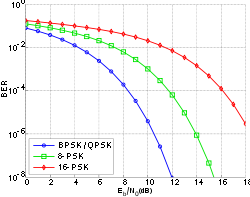
\includegraphics[width=0.7\linewidth]{BER_wiki.png} \\ Теоретическая зависимость}
		\end{minipage}
		\hfill
		\begin{minipage}[h]{0.49\linewidth}
			\center{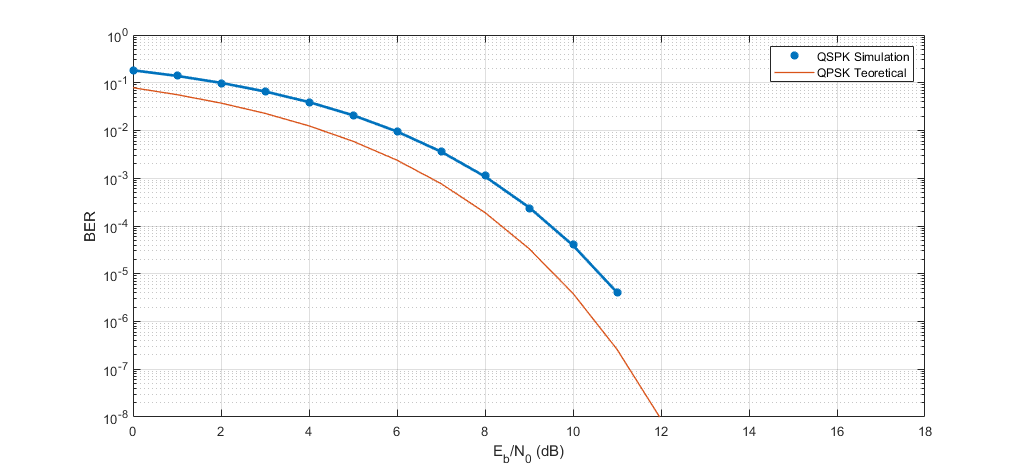
\includegraphics[width=0.9\linewidth]{qpsk_ber.png} \\ Модель ретранслятора}
		\end{minipage}
		\caption{Вероятность ошибки на бит (BER) в зависимости от $\frac{Eb}{N0}$ в dB}
		\label{fig:model20}
	\end{figure}


\begin{onehalfspace}


Системы ретрансляции способны передавать различные типы сигналов, и работать в разных диапазонах частот. Данная модель может быть применена при моделировании систем связи. В данном примере, идёт моделирование передачи данных, при разных значениях выходных мощностей сигналов абонента и базовой станции, при этом находящихся в предельной зоне видимости ретранслятора. Рисунок 21 демонстрирует состояния спектров сигналов, качественно это оценивается, как соответствие сигнала от базовой станции и ответного ему сигнала от абонента. Это позволяет оценивать минимальную выходную мощность сигнала.

Однако в случае, когда усиление сигнала недостаточно и мощности не хватает, чтобы достичь предела чувствительности приёмника ретранслятора, происходит потеря полезного сигнала, что демонстрируется на рисунках 22 и 23.
\end{onehalfspace}

 \begin{figure}[h!]
\centering
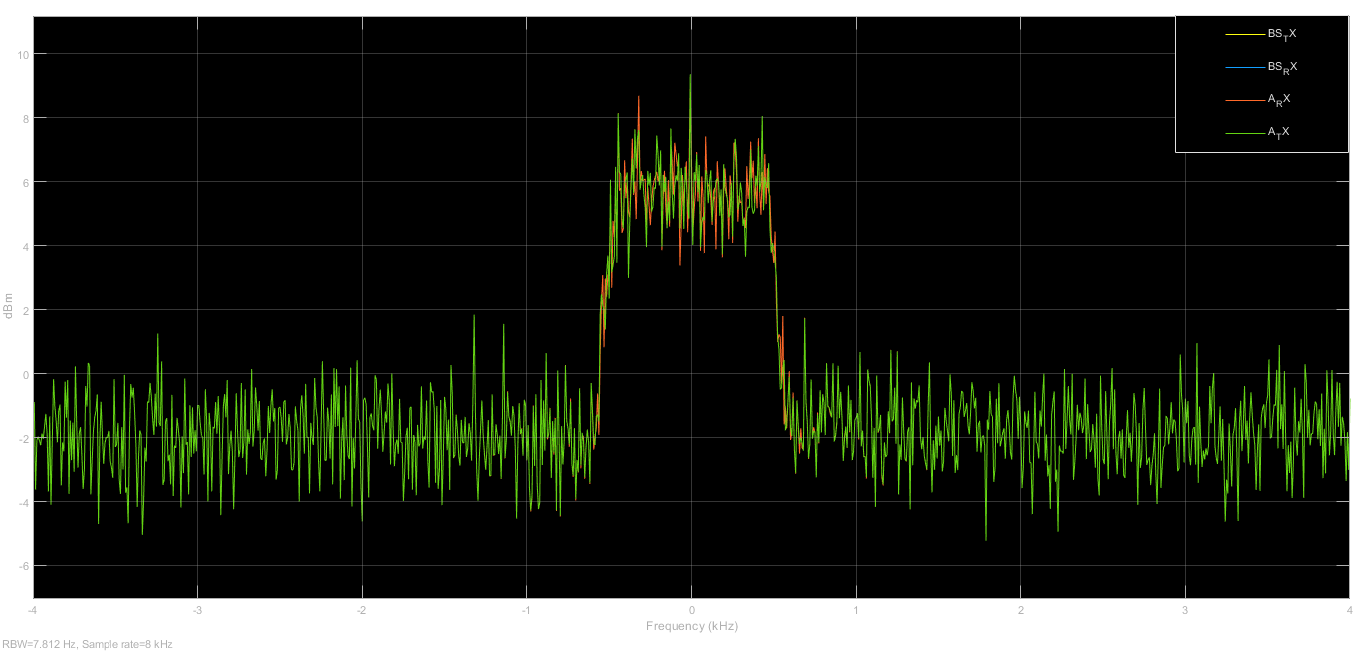
\includegraphics[width=1\linewidth]{Spectrum_Retranslation.png}
\caption{Спектры сигналов с расчитанным усилением}
\label{fig:model23}
\end{figure}
 \begin{figure}[h!]
\centering
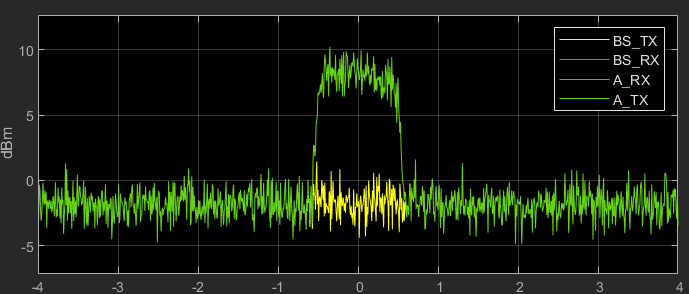
\includegraphics[width=0.95\linewidth]{umer_signal_sid.png}
\caption{Спектры сигналов при наличии ослабления в канале <<базовая станция — ретранслятор>>}
\label{fig:model23}
\end{figure}

\begin{figure}[H]
\begin{minipage}[h]{0.47\linewidth}
\center{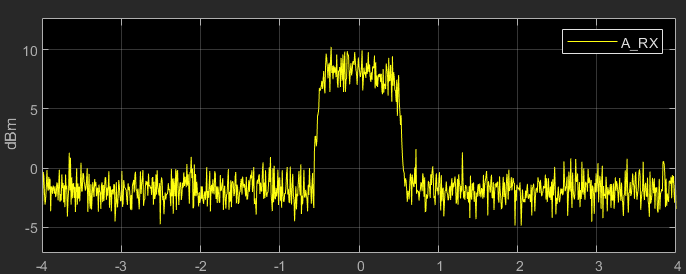
\includegraphics[width=1\linewidth]{umer_signal_a_rx.png}}  1) Спектр принятого сигнала абонента;  \\
\end{minipage}
\hfill
\begin{minipage}[h]{0.47\linewidth}
\center{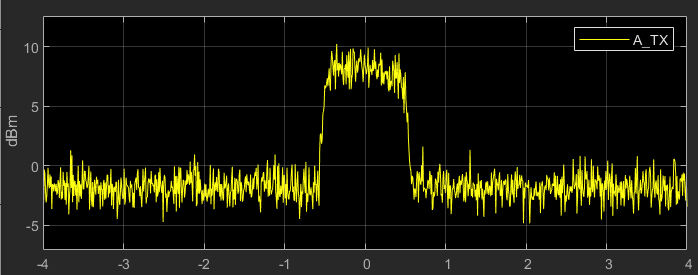
\includegraphics[width=1\linewidth]{umer_signal_a_tx.png}} \\2) Спектр отправленного сигнала абонента;
\end{minipage}
\vfill
\begin{minipage}[h]{0.47\linewidth}
\center{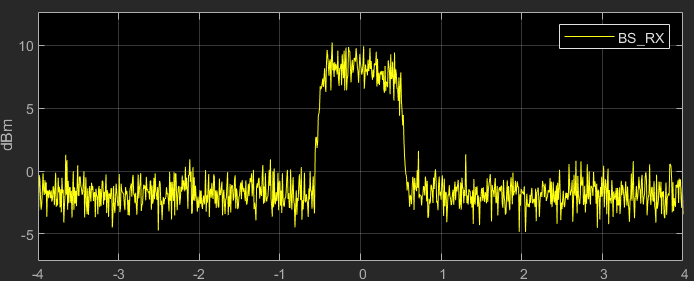
\includegraphics[width=1\linewidth]{umer_signal_b_rx.png} 3) Спектр принятого сигнала базовой станции; \\
\end{minipage}
\hfill
\begin{minipage}[h]{0.47\linewidth}
\center{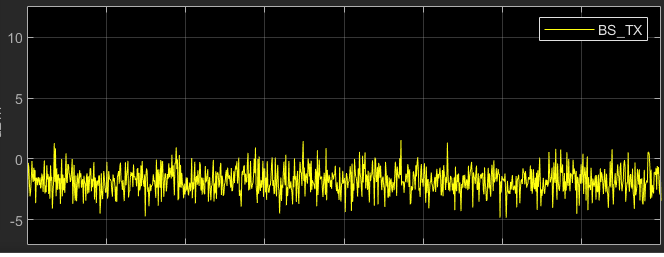
\includegraphics[width=1\linewidth]{umer_signal_b_tx.png}}  4) Спектр отправленного сигнала базовой станции; \\
\end{minipage}
\caption{Спектры сигналов в канале <<базовая станция — абонент>>}
\label{fig:model24}
\end{figure}



\begin{onehalfspace}

Также модель позволяет оценивать предельные физические расстояния между станциями. К примеру, из-за ослабления сигнала, а также из-за несовершенств оборудования, таких как нестабильности характеристик
элементов системы, параметры сигнала изменяются относительно расчётных параметров отправленного сигнала, что приводит к ухудшению качества принимаемого сигнала, ухудшению
синхронизации и ослаблению сигнала. Это влияние на сигнал моделируется блоком потерь энергии в свободном пространстве, а также блоком смещения фазы и частоты. Для увеличения дальности передачи, уже ослабленный сигнал, получаемый ретранслятором, усиливается, и пересылается абоненту, как почти точная копия исходного сигнала базовой станции. Определение максимальной длины каналов связи (каналы <<базовая станция — ретранслятор>> и <<абонент — ретранслятор>>) необходимо, чтобы гарантировать, корректность и распознаваемость принятого сигнала. При задании значения выходной мощности сигнала на приёмнике можно моделировать процесс окончательного затухания и предельное расстояние для передачи валидных данных. Рисунок 24 демонстрирует вид спектров модельных сигналов передачи абонента и ретранслятора, видно изменение в спектре после ослабления сигнала в канале, фазового и частотного сдвига. 
\end{onehalfspace}

\begin{figure}[h]
		\begin{minipage}[h]{0.49\linewidth}
			\center{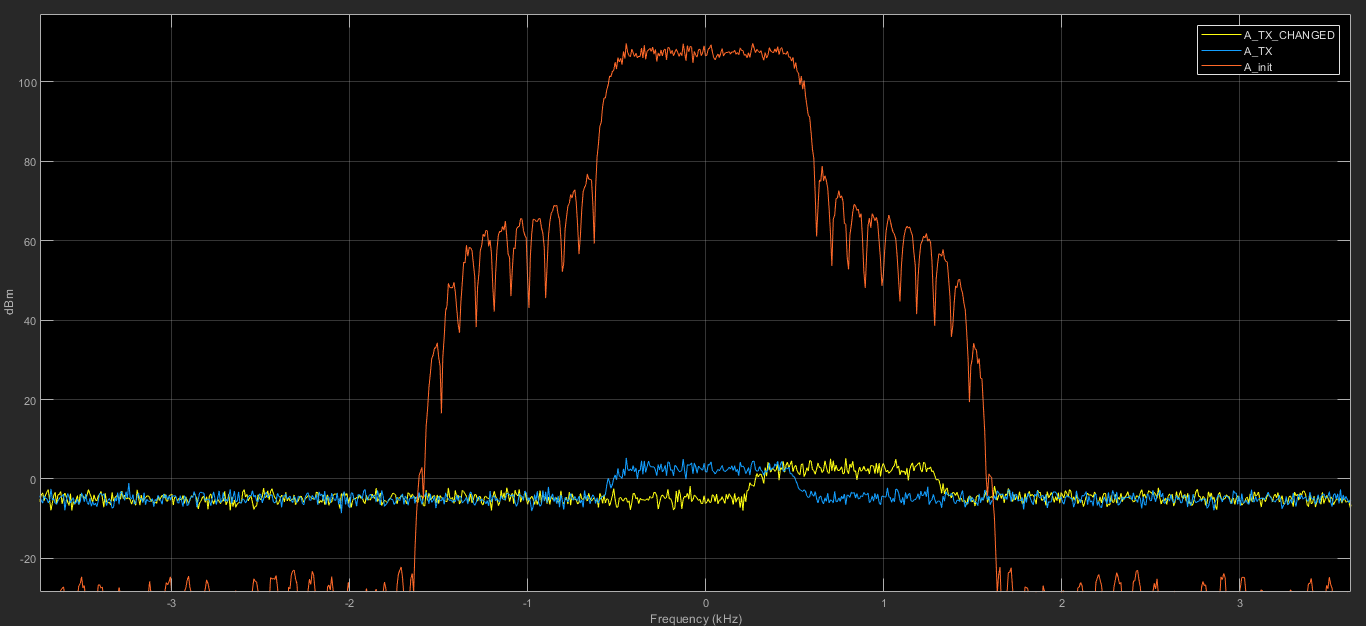
\includegraphics[width=1\linewidth]{a_inside_chan.png}} \\ абонент}
		\end{minipage}
		\hfill
		\begin{minipage}[h]{0.49\linewidth}
			\center{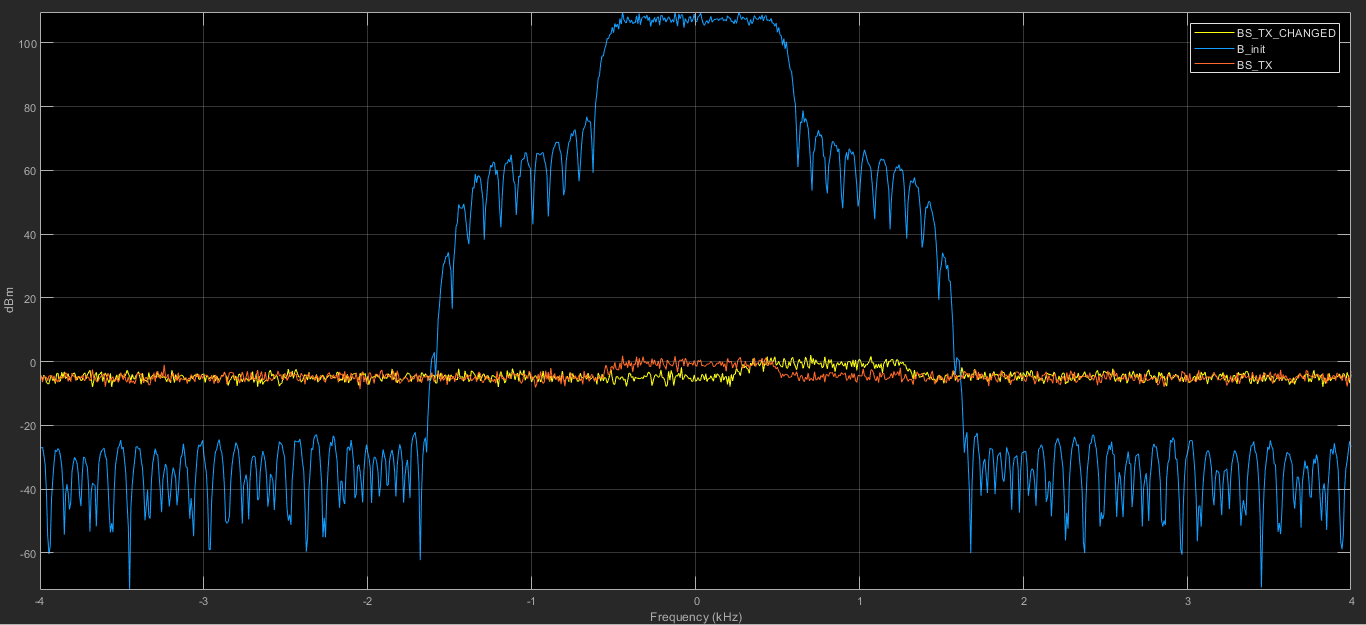
\includegraphics[width=1\linewidth]{bs_inside_chann.png}} \\ базовая станция}
		\end{minipage}
		\caption{Спектры модельных сигналов передачи}
		\label{fig:model20}
	\end{figure}


\begin{onehalfspace}
В обратную сторону, при заданных расстояниях, модель позволяет оценивать значение необходимых выходных мощностей потребителей базовая станция и абонент для связи с ретранслятором.

Значение величины запаса энергии канала позволяет оценивать, насколько система удовлетворяет поставленным к ней требованиям. Это значение может указывать на возможные аппаратные ограничения и, с помощью моделирования, можно разрабатывать способы их компенсировать за счет других частей канала. В таблице 1 указаны возможные значения для заданного расстояния.

\begin{center}
		\begin{tabular}{|p{5cm}|p{6.5cm}|}
			\hline
			  Модель & Запас мощности канала [dB], 
  Расстояние [км] \\
			\hline
			абонент (TX) & $26.973, 50$ \\
			\hline
			абонент (RX) & $26.973, 50$\\
			\hline
			базовая станция (TX) & $27.134, 50$ \\	
			\hline
   базовая станция (RX) & $26.654, 50$\\
			\hline
		\end{tabular}
		\label{table:1}
  \end{center}
  \begin{center}
  Таблица 1 — Моделирование запаса мощности каналов <<базовая станция — ретранслятор>>, <<абонент — ретранслятор>>
	\end{center}


\end{onehalfspace}







\section*{\large{3.4 Результаты моделирования абонента}}
\addcontentsline{toc}{section}{3.4 Результаты моделирования абонента}
\begin{onehalfspace}
Исследуемым фактором является сигнал на модуле абонента. Отследить это влияние на значение результата можно сравнением одиночной работы модуля в режиме одновременного приёма и передачи, и работы в комплексе с остальными модулями, в этом случае ping-сигнал посылается абонентом, с ожидание ответа базовой станции. Рисунок 25 демонстрирует эти результаты для первого описанного случая, сигнал приходящий на приёмник абонента, за счёт искажений складывается со своими копиями, имеющими отличную амплитуду и частоту, далее, внутри модуля происходит выделение полезного сигнала. он отображает соответствие модельных данных значения BER ожидаемым теоритическим, в канале $A\_bb\_tx - A\_bb\_rx$ ($A\_bb\_tx\_valid - A\_bb\_rx\_valid$), с помощью расчёта показателя достоверности приема двоичных символов.
\end{onehalfspace}

\begin{figure}[h]
		\begin{minipage}[h]{0.49\linewidth}
			\center{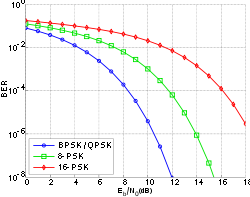
\includegraphics[width=0.7\linewidth]{BER_wiki.png} \\ Теоретическая зависимость}
		\end{minipage}
		\hfill
		\begin{minipage}[h]{0.49\linewidth}
			\center{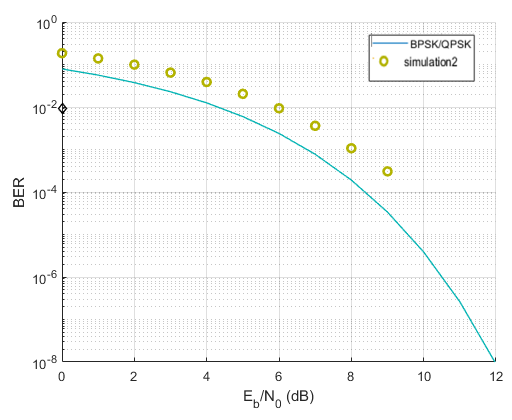
\includegraphics[width=0.8\linewidth]{realPSKa.png} \\ Модель абонента}
		\end{minipage}
		\caption{Вероятность ошибки на бит (BER) в зависимости от $\frac{Eb}{N0}$ в dB}
		\label{fig:model24}
\end{figure}

\begin{onehalfspace}
Аналогично 2.1 базовая станция BER показывает частоту возникновения ошибки в передаче данных по радиоканалу, являясь показателем качества связи в канале радиосвязи <<абонент — ретранслятор>>. Спектр полученного сигнала будет зависеть от этих процессов обработки. Рисунок 26 демонстрирует спектры сигналов при моделировании сценария ping, с компенсацией задержек за счёт внутреннего устройства модуля (фильтры, модулирующие блоки), полученной в канале валидности $A\_bb\_tx\_valid - A\_bb\_rx\_valid$.
\end{onehalfspace}

\begin{figure}[h]
		\begin{minipage}[h]{0.49\linewidth}
			\center{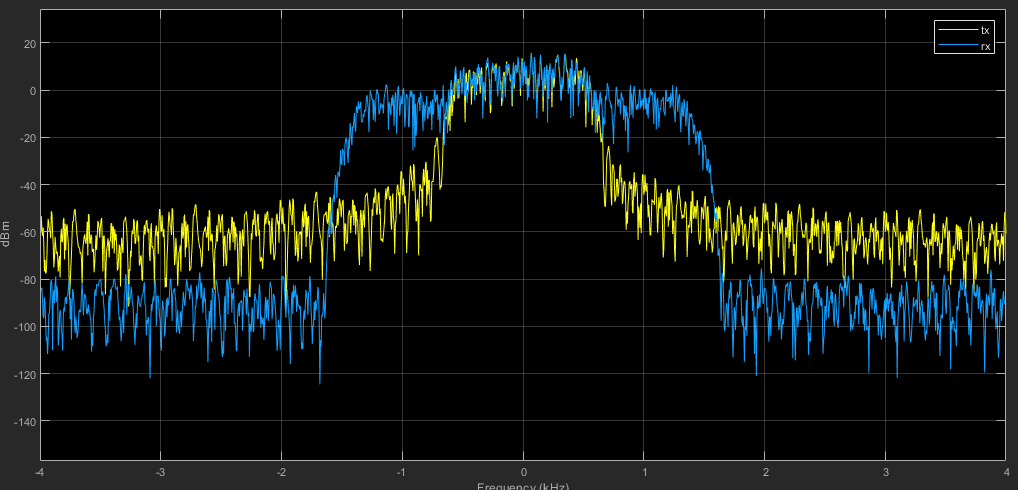
\includegraphics[width=0.8\linewidth]{abo_spec.png} \\  Спектры принятого и отправленного ping-сигнала абонента}
		\end{minipage}
		\hfill
		\begin{minipage}[h]{0.49\linewidth}
			\center{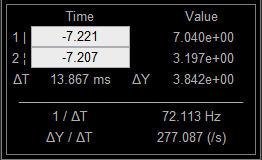
\includegraphics[width=0.7\linewidth]{abo_det.png} \\ Временные задержки модели, полученные мониторингом линии валидности}
		\end{minipage}
		\caption{Результат моделирования собственного сигнала}
		\label{fig:model25}
	\end{figure}


